\documentclass[landscape]{baposter}
\usepackage{amsmath}
\usepackage{amsxtra}
\usepackage{algorithmic}
\usepackage{bbm}

\usepackage[vlined]{algorithm2e}
\usepackage{times}
\usepackage{calc}
\usepackage{url}
\usepackage{graphicx}
\usepackage{amsmath}
\usepackage{amsxtra}
\usepackage{amssymb}
\usepackage{relsize}
\usepackage{multirow}
\usepackage{booktabs}

\usepackage{graphicx}
\usepackage{multicol}
\usepackage[T1]{fontenc}
\usepackage{ae}

\newcommand*{\add}{\mbox{\bf add}} 
\newcommand*{\open}{\mbox{\bf open}} 
\newcommand*{\close}{\mbox{\bf close}} 
\newcommand*{\ex}{\mbox{\rm E}} 
\newcommand*{\pr}{\mbox{\rm Pr}} 
\newcommand*{\range}{\mbox{\rm range}} 
\newcommand*{\rank}{\mbox{\rm rank}} 
\newcommand*{\sgn}{\mbox{\rm sign}} 
\newcommand*{\var}{\mbox{\rm Var}} 
\newcommand*{\diag}{\mbox{\rm diag}} 
\newcommand*{\epi}{\epsilon} 
\newcommand*{\QED}{\ \hfill\rule[-2pt]{6pt}{12pt} \medskip}
\newcommand*{\supp}{\mbox{\rm supp}} 

\newcommand*{\grad}{\nabla}
\newcommand*{\half}{\frac{1}{2}}
\newcommand*{\inv}{^{-1}}
\newcommand*{\0}{\mathbf{0}}
\newcommand*{\1}{\mathbf{1}}
\newcommand*{\E}{\ensuremath{\operatorname{E}}}
\newcommand*{\maximize}{\text{maximize}}
\newcommand*{\minimize}{\text{minimize}}
\newcommand*{\st}{\text{subject to}}
\newcommand*{\R}{\mathbb{R}}
\newcommand*{\matlab}{{\sc Matlab}}



\newcommand{\abs}[1]{\left\vert #1 \right\vert}
\newcommand{\bigo}[1]{\mathcal{O} \left( #1 \right)}
\newcommand{\cov}[2]{\ensuremath{\operatorname{Cov}\left( #1, #2\right)}}
\newcommand{\Ex}[2][]{\ensuremath{\E_{#1} \left[ #2 \right]}}
\newcommand{\norm}[1]{\left\lVert\,#1\,\right\rVert}
\newcommand{\bmat}[1]{\begin{bmatrix}#1\end{bmatrix}}
\newcommand{\pmat}[1]{\begin{pmatrix}#1\end{pmatrix}}
\newcommand{\smallmat}[1]{\left (\begin{smallmatrix}#1\end{smallmatrix} \right)}
\newcommand{\vb}[1]{\mathbf{#1}}

\renewcommand{\P}{\ensuremath{\operatorname{P}}}
\renewcommand{\Pr}[2][]{\ensuremath{\P_{#1} \left \{ #2 \right \}}}

%%%%%%%%%%%%%%%%%%%%%%%%%%%%%%%%%%%%%%%%%%%%%%%%%%%%%%%%%%%%%%%%%%%%%%%%%%%%%%%
 % Multicol Settings
 %%%%%%%%%%%%%%%%%%%%%%%%%%%%%%%%%%%%%%%%%%%%%%%%%%%%%%%%%%%%%%%%%%%%%%%%%%%%%%%%
 \setlength{\columnsep}{0.7em}
 \setlength{\columnseprule}{0mm}

\font\dsfnt=dsrom12


 \begin{document}
\begin{poster}
  {
  % Show grid to help with alignment grid=no,
	% Column spacing
	colspacing=0.7em,
	% Color style
	headerColorOne=cyan!20!white!90!black,
	borderColor=cyan!30!white!90!black,
	% Format of textbox
 	textborder=faded,
	% Format of text header
	headerborder=open, headershape=roundedright, background=none,
	bgColorOne=cyan!10!white, headerheight=0.12\textheight}
%HI university logo
   {
      
\includegraphics[height=0.12\textheight]{./images/SU_Seal_red.png}\\
   }
 %Title
  {
  Existence of Positive Equilibria for Mass Conserving and Mass-Action
	Chemical Reaction Networks with a 
	Single-Terminal-Linkage Class
  }
  %Authors
  {
 \vskip 2pt
  Santiago Akle,
   Onkar Dalal,
   Ronan Fleming, 
   Michael Saunders,
   Nicole Taheri,
   Yinyu Ye.
   }
%HI university logo
   {
      
\includegraphics[height=0.12\textheight]{./images/ui_1_rgb.eps}\\
   }
%Contribution
 \headerbox{Contributions}
 {
 name=contribution,column=0,row=0,span=2
 }
 {
 We show that if a chemical reaction network {\em conserves mass} and is formed by a single {\em terminal-linkage-class}, then
 there exists a positive steady state for the dynamic, regardless of the deficiency and choice of kinetic constants.
 We hope this analysis will yield insights about systems that achieve non-equilibrium steady states.
 }
 \headerbox{Chemical Reaction Networks}
 {
 name=cnets,column=0,span=1,below=contribution
 }
 {
\parskip 2pt 
We represent a reaction network by a weighted directed graph
$G(V,E)$ with each node denoting a complex and each directed edge
$i\rightarrow j$ denoting a reaction using $i$ to generate $j$ and weighted by
the positive reaction rate constant $k_{i\rightarrow j}$.

Let $A \in \R^{n
\times n}$ be the adjacency matrix of $G$, where
$A_{ij}=k_{i\rightarrow j}$, let  $D := \diag(A\1)$, where $\1$ is the
vector of all ones, let $A_k := A^T-D$ and 
$\Psi(c):\R^m_+\rightarrow \R^n$ be
\[\Psi_j(c) := \prod_i\,c_i^{Y_{ij}}.\] The
system of ODEs governing the reaction network can then be written as \[\dot{c} =
YA_k\Psi(c).\]

A steady state is a vector $0\leq c\in\R^m$ of concentrations, such that $YA_k\Psi(c)=0$ or equivalently, a pair
$(c,v)$, where $0\leq c\in\R^m$ and $v\in\R^n$ with
\begin{align} YA_kv &=0, \label{fb}\tag{FB} \\ \Psi(c)
  &= v. \label{mak}\tag{MA} \end{align}

Whenever $c>0$ we have that \[\log(v) = \log(\Psi(c)) = Y^T\log(c),\] then the conditions 
for a positive steady state are

\begin{align}
  YA_kv &=0 \tag{FB}, \\ 
   Y^T\log(c) &= \log(v). \label{mak-alt}\tag{MA-Log}
\end{align} 
}

\headerbox{Not only Complex Balance}
{name=cmplx, column=0,span=1,below=cnets}
{
Complex balance refers to steady states where $(v,c)$ satisfy
$A_kv=0$ and $\Psi(c)=v$. There can be more solutions to the system where
$A_kv \neq 0$ but $YA_kv=0$, and $\Psi(c)=v$. We prove the existence of positive 
steady states that are not necessarily complex balanced.
}


 \headerbox{Solutions as Fixed Points}
 {
 name = solsasfp, column=1, span=1,below=contribution
 } 
 {
 Let $\mu \in \R^m$ be a vector parameter.  Observe that if the parametric
convex optimization problem
\begin{align}
   \underset{v\in\R^n}{\minimize} &\quad v^TD(\log(v)-\1)    \notag
\\                     \st &\quad YD v = \mu  &:\ y \label{convex-fix}
\\                         &\quad v \ge 0                     \notag
\end{align}
has a strictly positive solution $v^\star(\mu)$, then the optimality condition
\begin{align}
   DY^T y^\star(\mu) &= D\log(v^\star)  \label{optcon}
 \end{align} 
 holds (here $y^\star(\mu)$ is the Lagrange multiplier of the equality
 constraint.)  Since $D$ is diagonal and strictly positive, this is equivalent
 to \eqref{mak-alt} with $y^\star(\mu)=\log(c^\star)$.


{\bf Is there a $\mu$ such that \eqref{fb} holds too?}

Note that the nonlinear program \eqref{convex-fix} is strictly convex, so for any
feasible $\mu$ there is a unique minimizer $v^\star(\mu).$
Define the function 
\begin{equation}  \label{mapping}
	 f(\mu) := YA^Tv^\star(\mu).  \end{equation}
If $\hat\mu$ is a fixed point of $f: \R^m \rightarrow \R^m$, then the linear
equality constraint in \eqref{convex-fix} implies
\[
   YDv^\star(\hat\mu) = \hat\mu = YA^Tv^\star(\hat\mu),
\]
or, equivalently,
\[
   Y(D-A^T)v^\star(\hat\mu) = -Y A_k v^\star(\hat\mu) = 0.
\]
Therefore at $\hat\mu$ both \eqref{mak-alt} and \eqref{fb} hold, and if
$v^\star(\hat\mu)$ then $c^\star = \exp(y^\star(\hat\mu))$ will be 
a steady state.
 }

 \headerbox{Existence and computation of solutions}
 {
 name = fp, column=2,row=0, span=2
 }
 {
 }

 \headerbox{Necessary Conditions}
 {
 name=necessary,column=2,below=fp
 }
 {
 A chemical reaction network will be {\em mass-conserving} if, as the dynamics
 of the system develop, the total amount of mass stays constant. If $w_i$ is
 the relative mass of species $i$ the value of $\sum_i w_i c_i(t)$ must be
 constant, therefore $\sum_i w_i \dot c(t) = 0$, which implies that
 $w^TYA_k\Psi(c)=0$. We term a network {\em mass-conserving} if there
 exists a strictly positive vector $w\in\R^m$ such that $w^TYA_k = 0$.
(This implies that $w^TYA^T = w^TYD$.)

A chemical network is formed by a {\em single-terminal-linkage} class if there
is a directed path from every complex in the graph to every other. Intuitively
this will imply that if the concentration of one complex is positive then all
the reactions that transform it will occur. In turn this means that the
concentration of their products will be positive. Since the network is strongly
connected this will cascade to all complexes and define a positive equilibrium.
}

 \headerbox{Proof}
 {
 name=proof,column=2,below=necessary
 }
 {

Brouwer's theorem states that a continuous mapping from
a compact and convex set into itself must have a fixed point.

We select an arbitrary constant $\gamma>0$ and define the set
\[\Omega := \left\{ \mu:  e^T\mu = \gamma,\, \mu=Y\eta ,\,\eta\geq0  \right\}.\] This 
set will make problem \eqref{convex-fix} feasible and is also compact and convex.

Since matrices $Y$ and $A^T$ have nonnegative entries and $v^\star$ is nonnegative, then
$f(\mu)\geq0$. Also by the constraint in problem \ref{convex-fix},
$w^Tf(\mu) = w^TYA^Tv^\star(\mu) = w^TYDv^\star(\mu) = \gamma.$ Therefore $f(\mu)$ is in $\Omega$ and 
a fixed point $\hat\mu$ must exist.

Because $0\notin \Omega$, we know $\hat\mu \neq 0$, so that $v^\star(\hat\mu)\neq 0$ and we can use the single-class 
hypothesis to establish that $v^\star(\hat\mu)>0$ (refer to \cite{yyy-saund} for details).

 }

 \headerbox{Computing the solutions}
 {name=algo,column=3,below=fp}
 {
Given an initial point $0<v_0\in \Re^n$, and a small tolerance $\tau$, the algorithm proceeds as follows:
\begin{algorithmic}
  \STATE $v^\star \gets v_0$
  \STATE $\mu \gets YA^Tv^\star$
  \WHILE{$\|YA_k v^\star\|_\infty>\tau$}
  \STATE $v^\star\gets \text{unique solution of \eqref{convex-fix}} $
	\STATE $\mu \gets \frac{1}{2}\mu +\frac{1}{2}YA^Tv^\star$
  \ENDWHILE
  \label{fixpoint-alg}.
\end{algorithmic}

If $v^\star(\mu_k)>0$, and the minimization step is solved accurately, the optimality
conditions will imply that \[\|Y^T\lambda-\log(v^\star(\mu_k))\|_\infty \leq \delta,\] for some small $\delta$. 
If the iteration converges, at the fixed point \eqref{mak} will
be satisfied to a precision $\delta$ and \eqref{fb} to a precision $\tau$. Our experiments 
indicate that this algorithm converges even for multiple linkage class networks.

 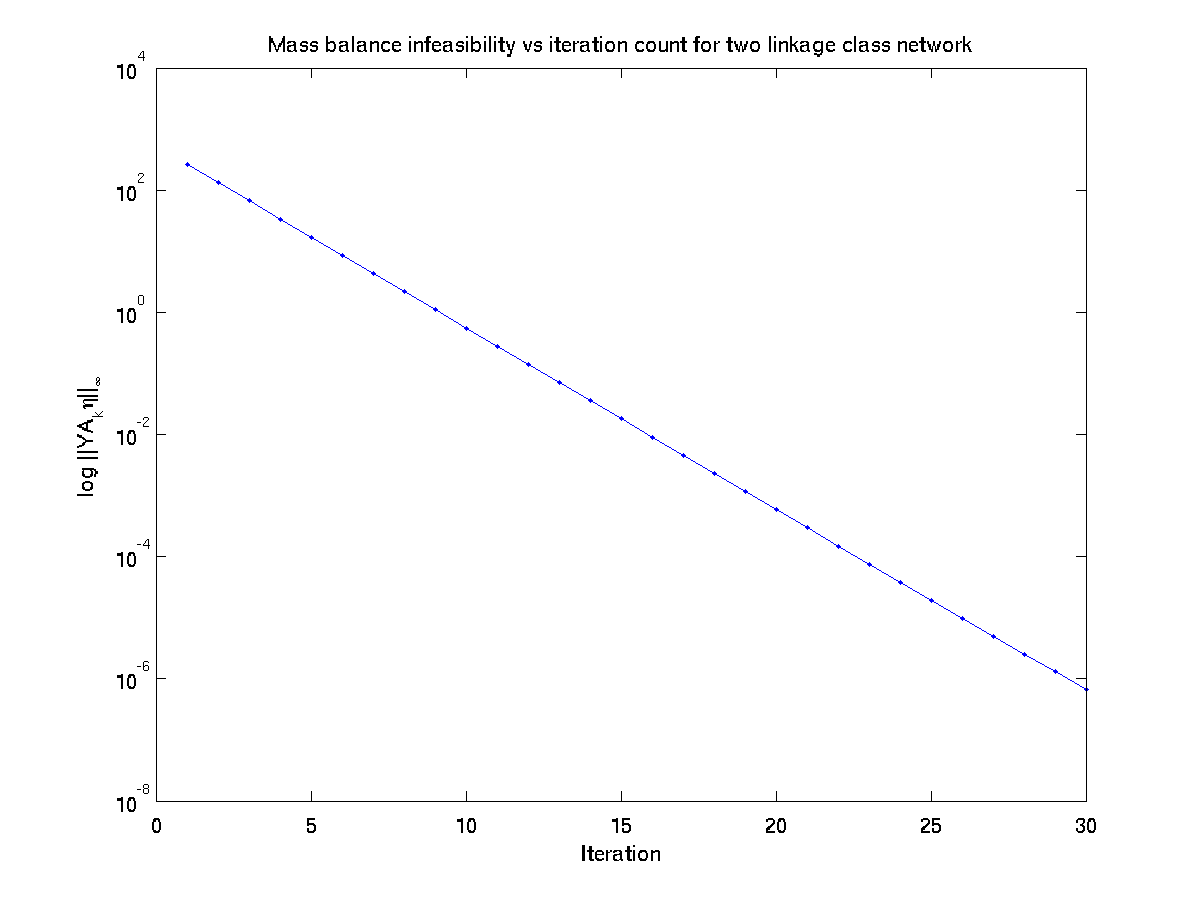
\includegraphics[scale=0.4]{./images/InfeasibilityVsIterationMultiple.png}
 \label{fig:typical-infeas-multiple}

 The above displays the sequence of infeasibilities
 $\|YA_kv_k\|_\infty$ when solving for a fixed point of a {\bf two} linkage class
 network with $50$ species and $500$ complexes where at most $10$ species
 participate in each complex.  We
 have observed this (apparently linear) convergence rate consistently over all
 generated networks {\bf regardless of the number of linkage classes}.
}

\headerbox{References}
{name=ref,column=1,span=2,below=proof}
{
\nocite{*} \bibliographystyle{plain} \bibliography{fixpointposter}{}
}



\end{poster}
\end{document}
